\documentclass[border=3pt]{standalone}
% Preâmbulo compartilhado pelos diagramas TikZ da aula
\usepackage[T1]{fontenc}
\usepackage[utf8]{inputenc}
\usepackage{lmodern}
\usepackage{amsmath}
\usepackage{xcolor}
\usepackage{tikz}
\usetikzlibrary{arrows.meta,angles,quotes,decorations.pathmorphing,calc,
                positioning,shapes.geometric,backgrounds,fit}

% Paleta (mesma dos SVGs originais)
\definecolor{dblue}{HTML}{2A5B8C}
\definecolor{dorange}{HTML}{B3541E}
\definecolor{dgreen}{HTML}{4A7C59}
\definecolor{dred}{HTML}{9C4B4B}
\definecolor{dcream}{HTML}{F4F1EA}
\definecolor{dshade}{HTML}{DDD7C9}

% Estilos comuns (prefixo d... para não colidir com chaves internas do pgf)
\tikzset{
  >={Stealth[length=2mm]},
  dguide/.style={gray!55, dashed, line width=0.4pt},
  daxis/.style={gray!60, line width=0.7pt, ->},
  dbody/.style={fill=black!3, draw=black!80, line width=1pt},
  dacc/.style={draw=dblue, line width=1pt},
  dlbl/.style={black!55, font=\small},
  dsub/.style={black!45, font=\footnotesize},
  dstate/.style={circle, draw=black!80, fill=dcream, line width=1pt,
                 minimum size=17mm, font=\large, inner sep=1pt},
  dobs/.style={circle, draw=black!80, fill=dshade, line width=1pt,
               minimum size=14mm, font=\large, inner sep=1pt},
  dbox/.style={rounded corners=2pt, draw=black!80, fill=dcream, line width=1pt,
               align=center, inner sep=6pt},
  dtrans/.style={->, dblue, line width=1pt},
  dmeas/.style={->, dorange, line width=1pt},
}

\begin{document}
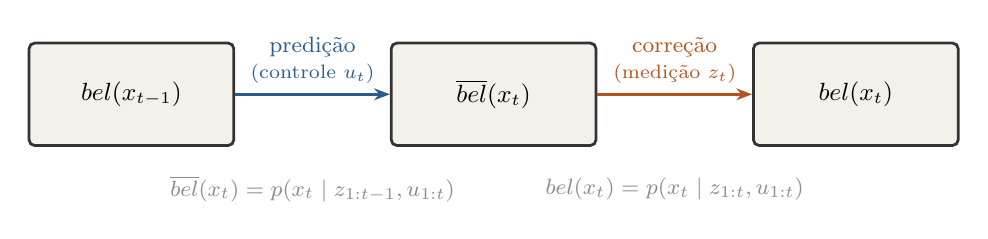
\begin{tikzpicture}[x=1cm,y=1cm]

  \node[dbox, minimum width=2.6cm, minimum height=1.3cm, font=\small]  (a) at (0,0)   {$bel(x_{t-1})$};
  \node[dbox, minimum width=2.6cm, minimum height=1.3cm, font=\small]  (b) at (4.6,0) {$\overline{bel}(x_t)$};
  \node[dbox, minimum width=2.6cm, minimum height=1.3cm, font=\small]  (c) at (9.2,0) {$bel(x_t)$};

  \draw[dtrans, line width=1.2pt] (a) -- node[above, dblue, font=\footnotesize, align=center]
        {predição\\\scriptsize (controle $u_t$)} (b);
  \draw[dmeas, line width=1.2pt] (b) -- node[above, dorange, font=\footnotesize, align=center]
        {correção\\\scriptsize (medição $z_t$)} (c);

  \node[dsub] at (2.3,-1.2) {$\overline{bel}(x_t)=p(x_t\mid z_{1:t-1},u_{1:t})$};
  \node[dsub] at (6.9,-1.2) {$bel(x_t)=p(x_t\mid z_{1:t},u_{1:t})$};

\end{tikzpicture}
\end{document}
